
% Due thursday

\documentclass{article}

\usepackage[utf8]{inputenc}

\usepackage{amsmath, bm}
\usepackage{graphicx}
\usepackage{amssymb}
\usepackage{float}
\usepackage{caption}
\usepackage{subcaption}
\usepackage{hyperref}
\usepackage{tikz}
\usepackage{layout}

\usepackage[margin=1in]{geometry}
\usepackage{listings}
\usepackage{xcolor}
\usepackage{color, colortbl}
\usepackage{textgreek}
\usepackage{mathrsfs}
\usepackage{savetrees}


\setlength{\parskip}{\baselineskip}%
\setlength{\parindent}{0pt}%
\linespread{0.9}


\definecolor{codegreen}{rgb}{0,0.6,0}
\definecolor{codegray}{rgb}{0.5,0.5,0.5}
\definecolor{codepurple}{rgb}{0.58,0,0.82}
\definecolor{backcolour}{rgb}{0.95,0.95,0.92}

\lstdefinestyle{mystyle}{
    backgroundcolor=\color{backcolour},   
    commentstyle=\color{codegreen},
    keywordstyle=\color{magenta},
    numberstyle=\tiny\color{codegray},
    stringstyle=\color{codepurple},
    basicstyle=\ttfamily\footnotesize,
    breakatwhitespace=false,         
    breaklines=true,                 
    captionpos=b,                    
    keepspaces=true,                 
    numbers=left,                    
    numbersep=5pt,                  
    showspaces=false,                
    showstringspaces=false,
    showtabs=false,                  
    tabsize=2
}

\lstset{style=mystyle}



\begin{document}

\title{GA3: Heat Exchanger Final Report}
\author{lwp26}
\date{June 2024}
\maketitle 


\section{Introduction}

The development of heat exchanger design software is incomplete without real world performance evaluation.
This report covers the assembly, testing and final performance of the assembled design chosen by our software compared to those selected and built by other groups.

\section{Results}

\subsection{Group E Assembly}
A major design flaw appeared due to not considering a 1mm gap for the outer O ring between inner and outer shell lengths which forced use to increase tube length by 3mm.
Another small issue was that the compression cage did not allow the the nozzles to be 60 degrees apart, as specified by the drawings.
The diameter for small O rings and tubes was 0.36mm smaller than the value of 10.92 mm defined in the handout which was caused by instead defining the angle to be 45 degrees, which was not the case.
This issue made it harder to assemble the tubes, but also provided a better seal between cold and hot sections.
% nozzle problems
% baffle and end cap assembly problems
These issues immidiately highlight differences which were not accounted for in the uncertainty analysis in the previous performance report.

\begin{figure}[H]
    \centering
    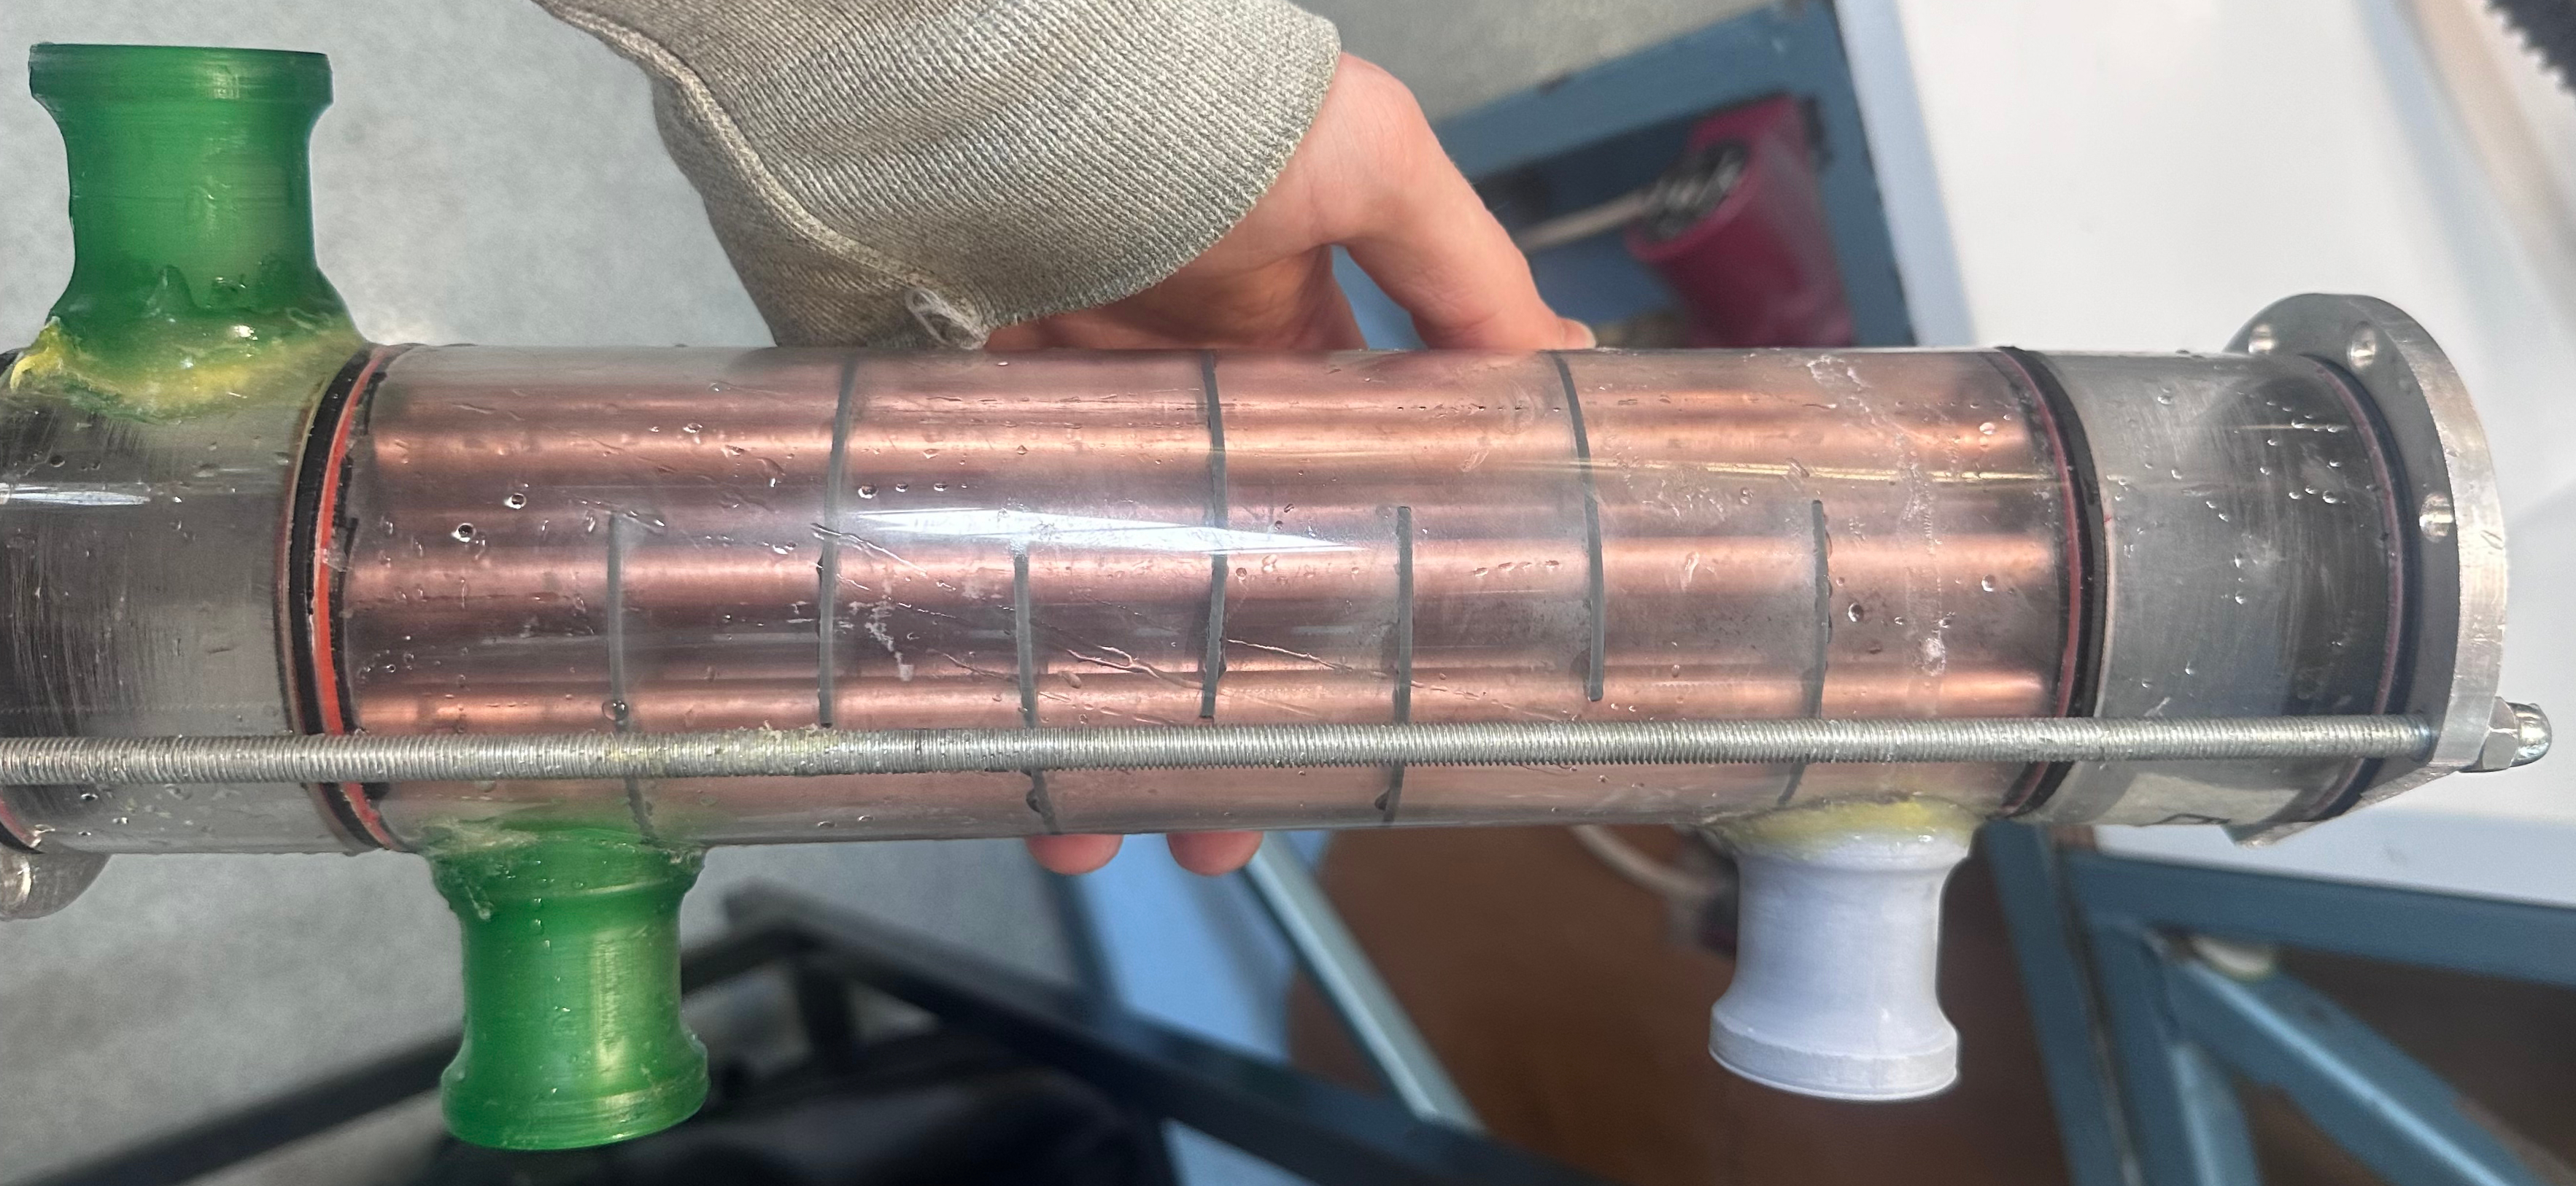
\includegraphics[width=0.5\textwidth]{final_tested.jpg}
    \caption{Final tested heat exchanger}
    \label{fig:heat_exchanger}
\end{figure}

\section{Results}

\iffalse
\begin{figure}[H]
    \centering
    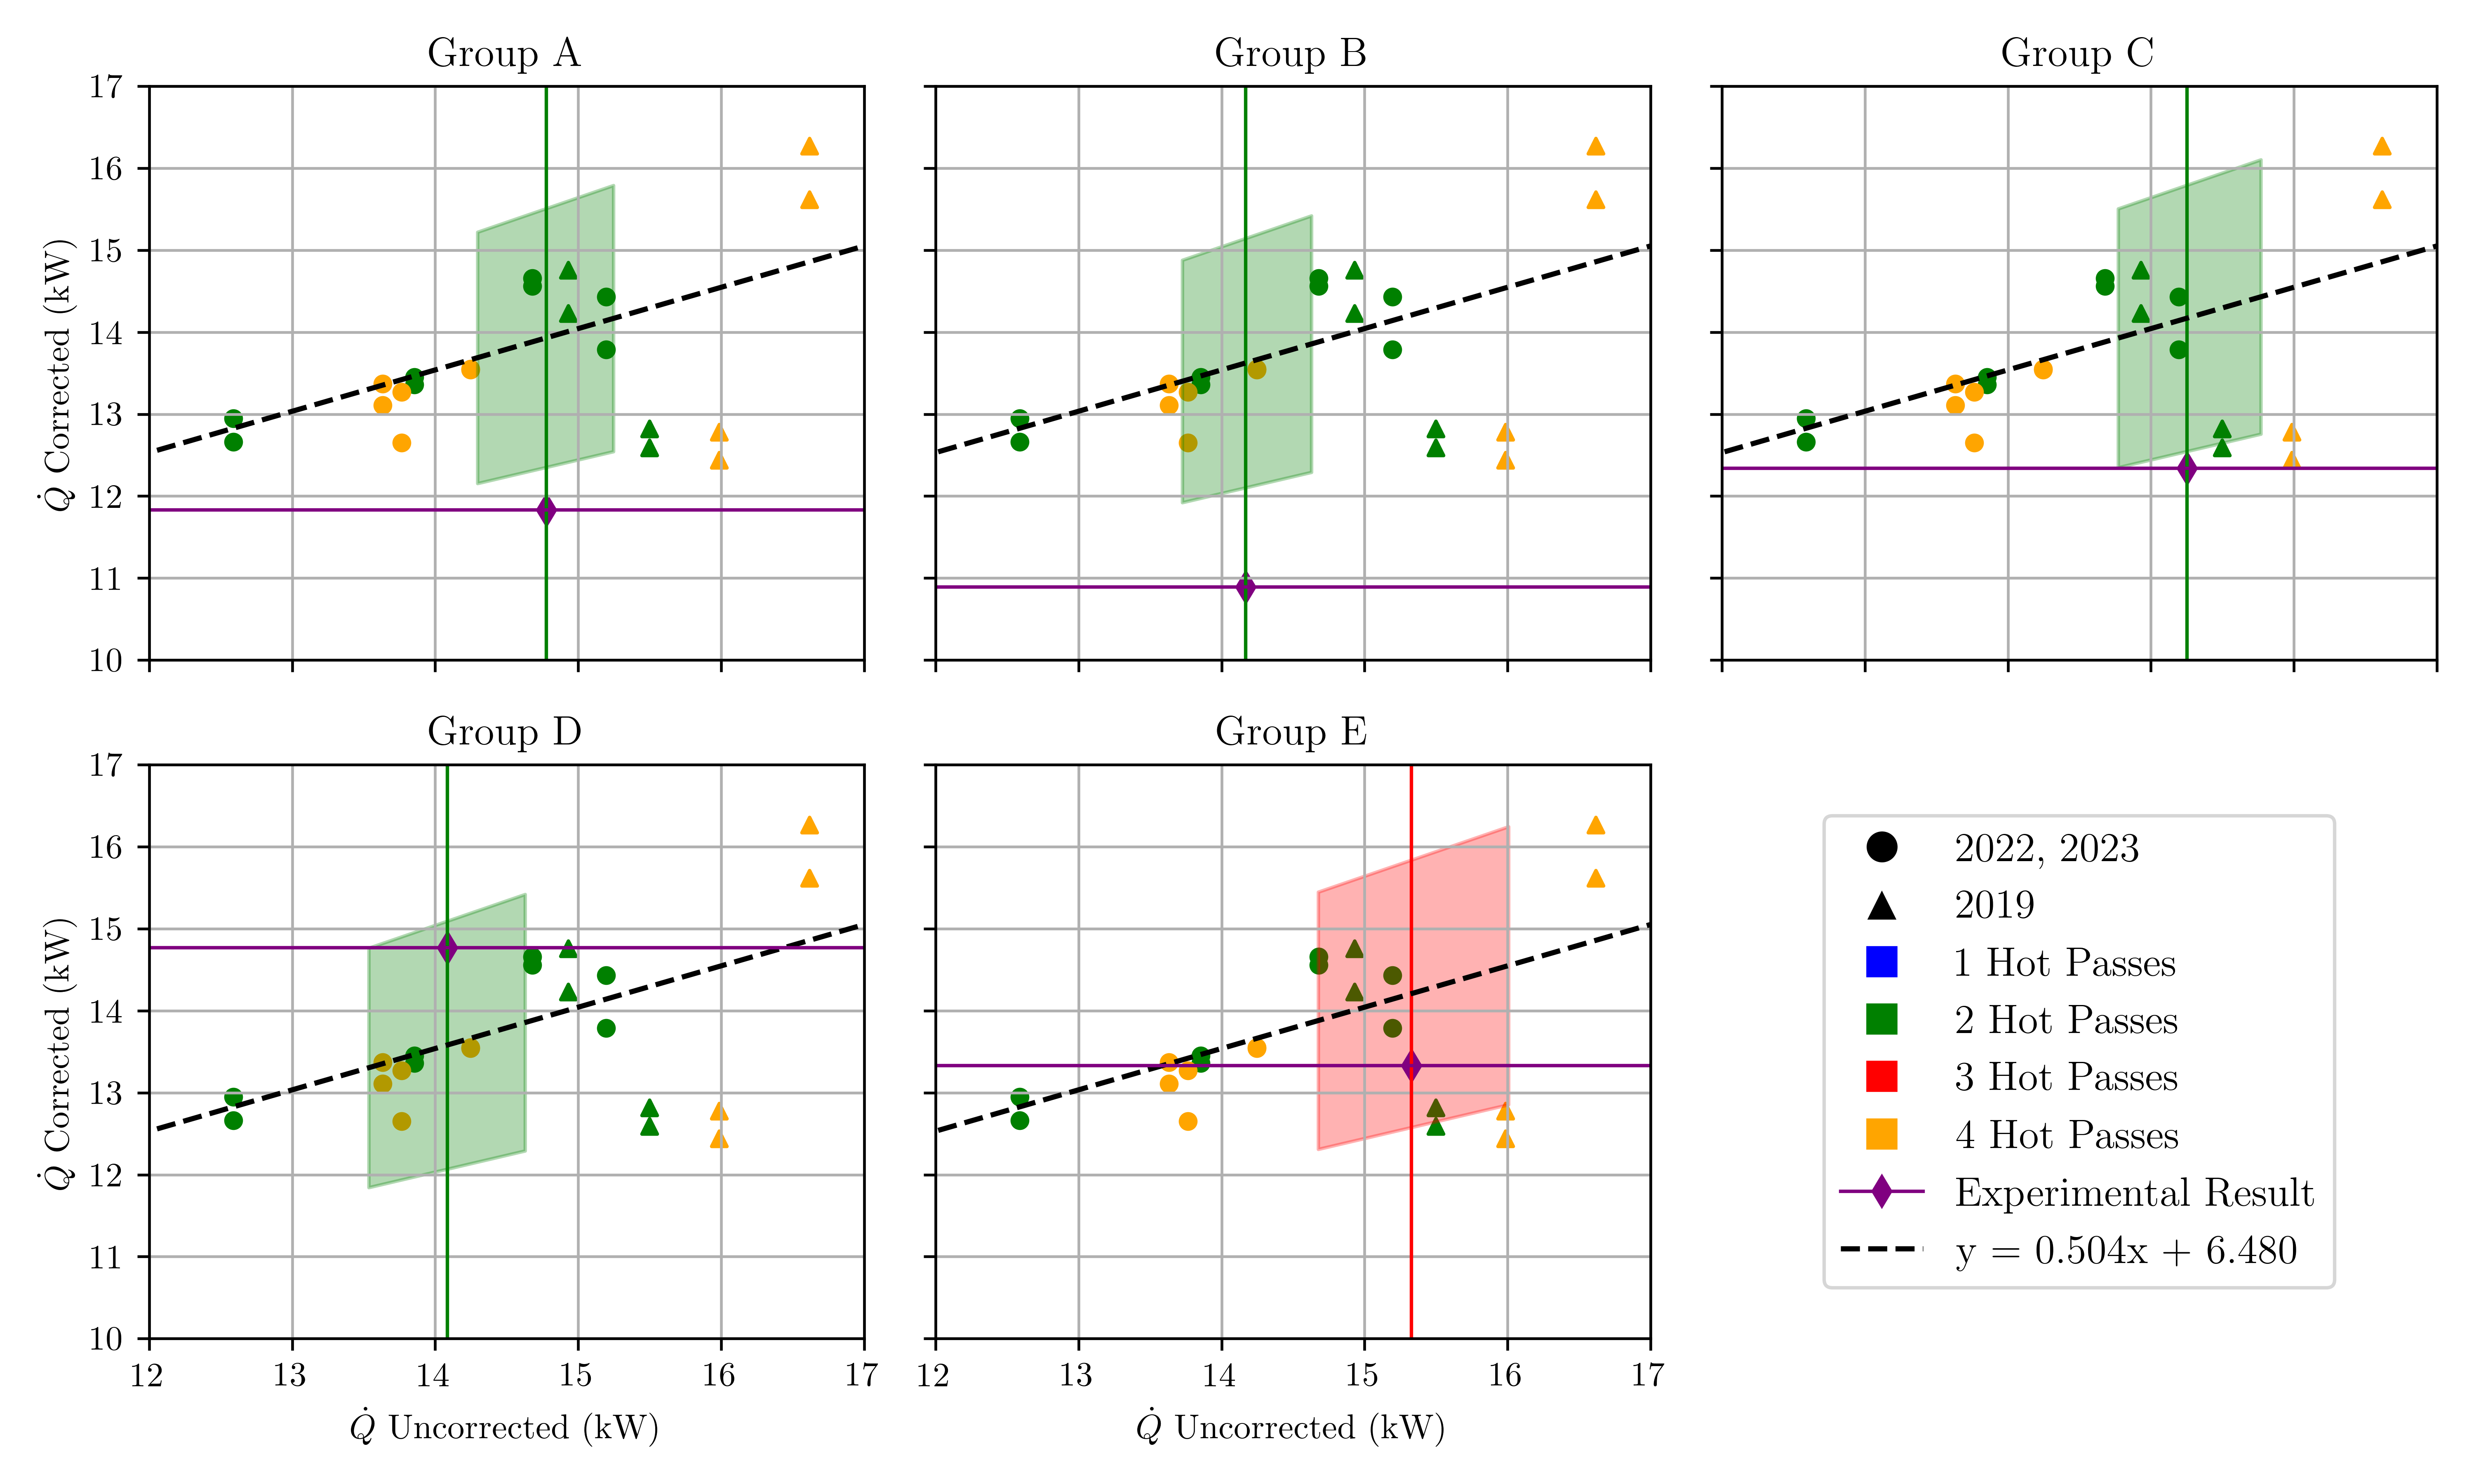
\includegraphics[width=0.9\textwidth]{Qdot_result_bands.png}
    \caption{Qdot results}
    \label{fig:Qdot_results}
\end{figure}
\fi

\begin{figure}[H]
    \centering
    \begin{subfigure}{0.6\textwidth}
        \centering
        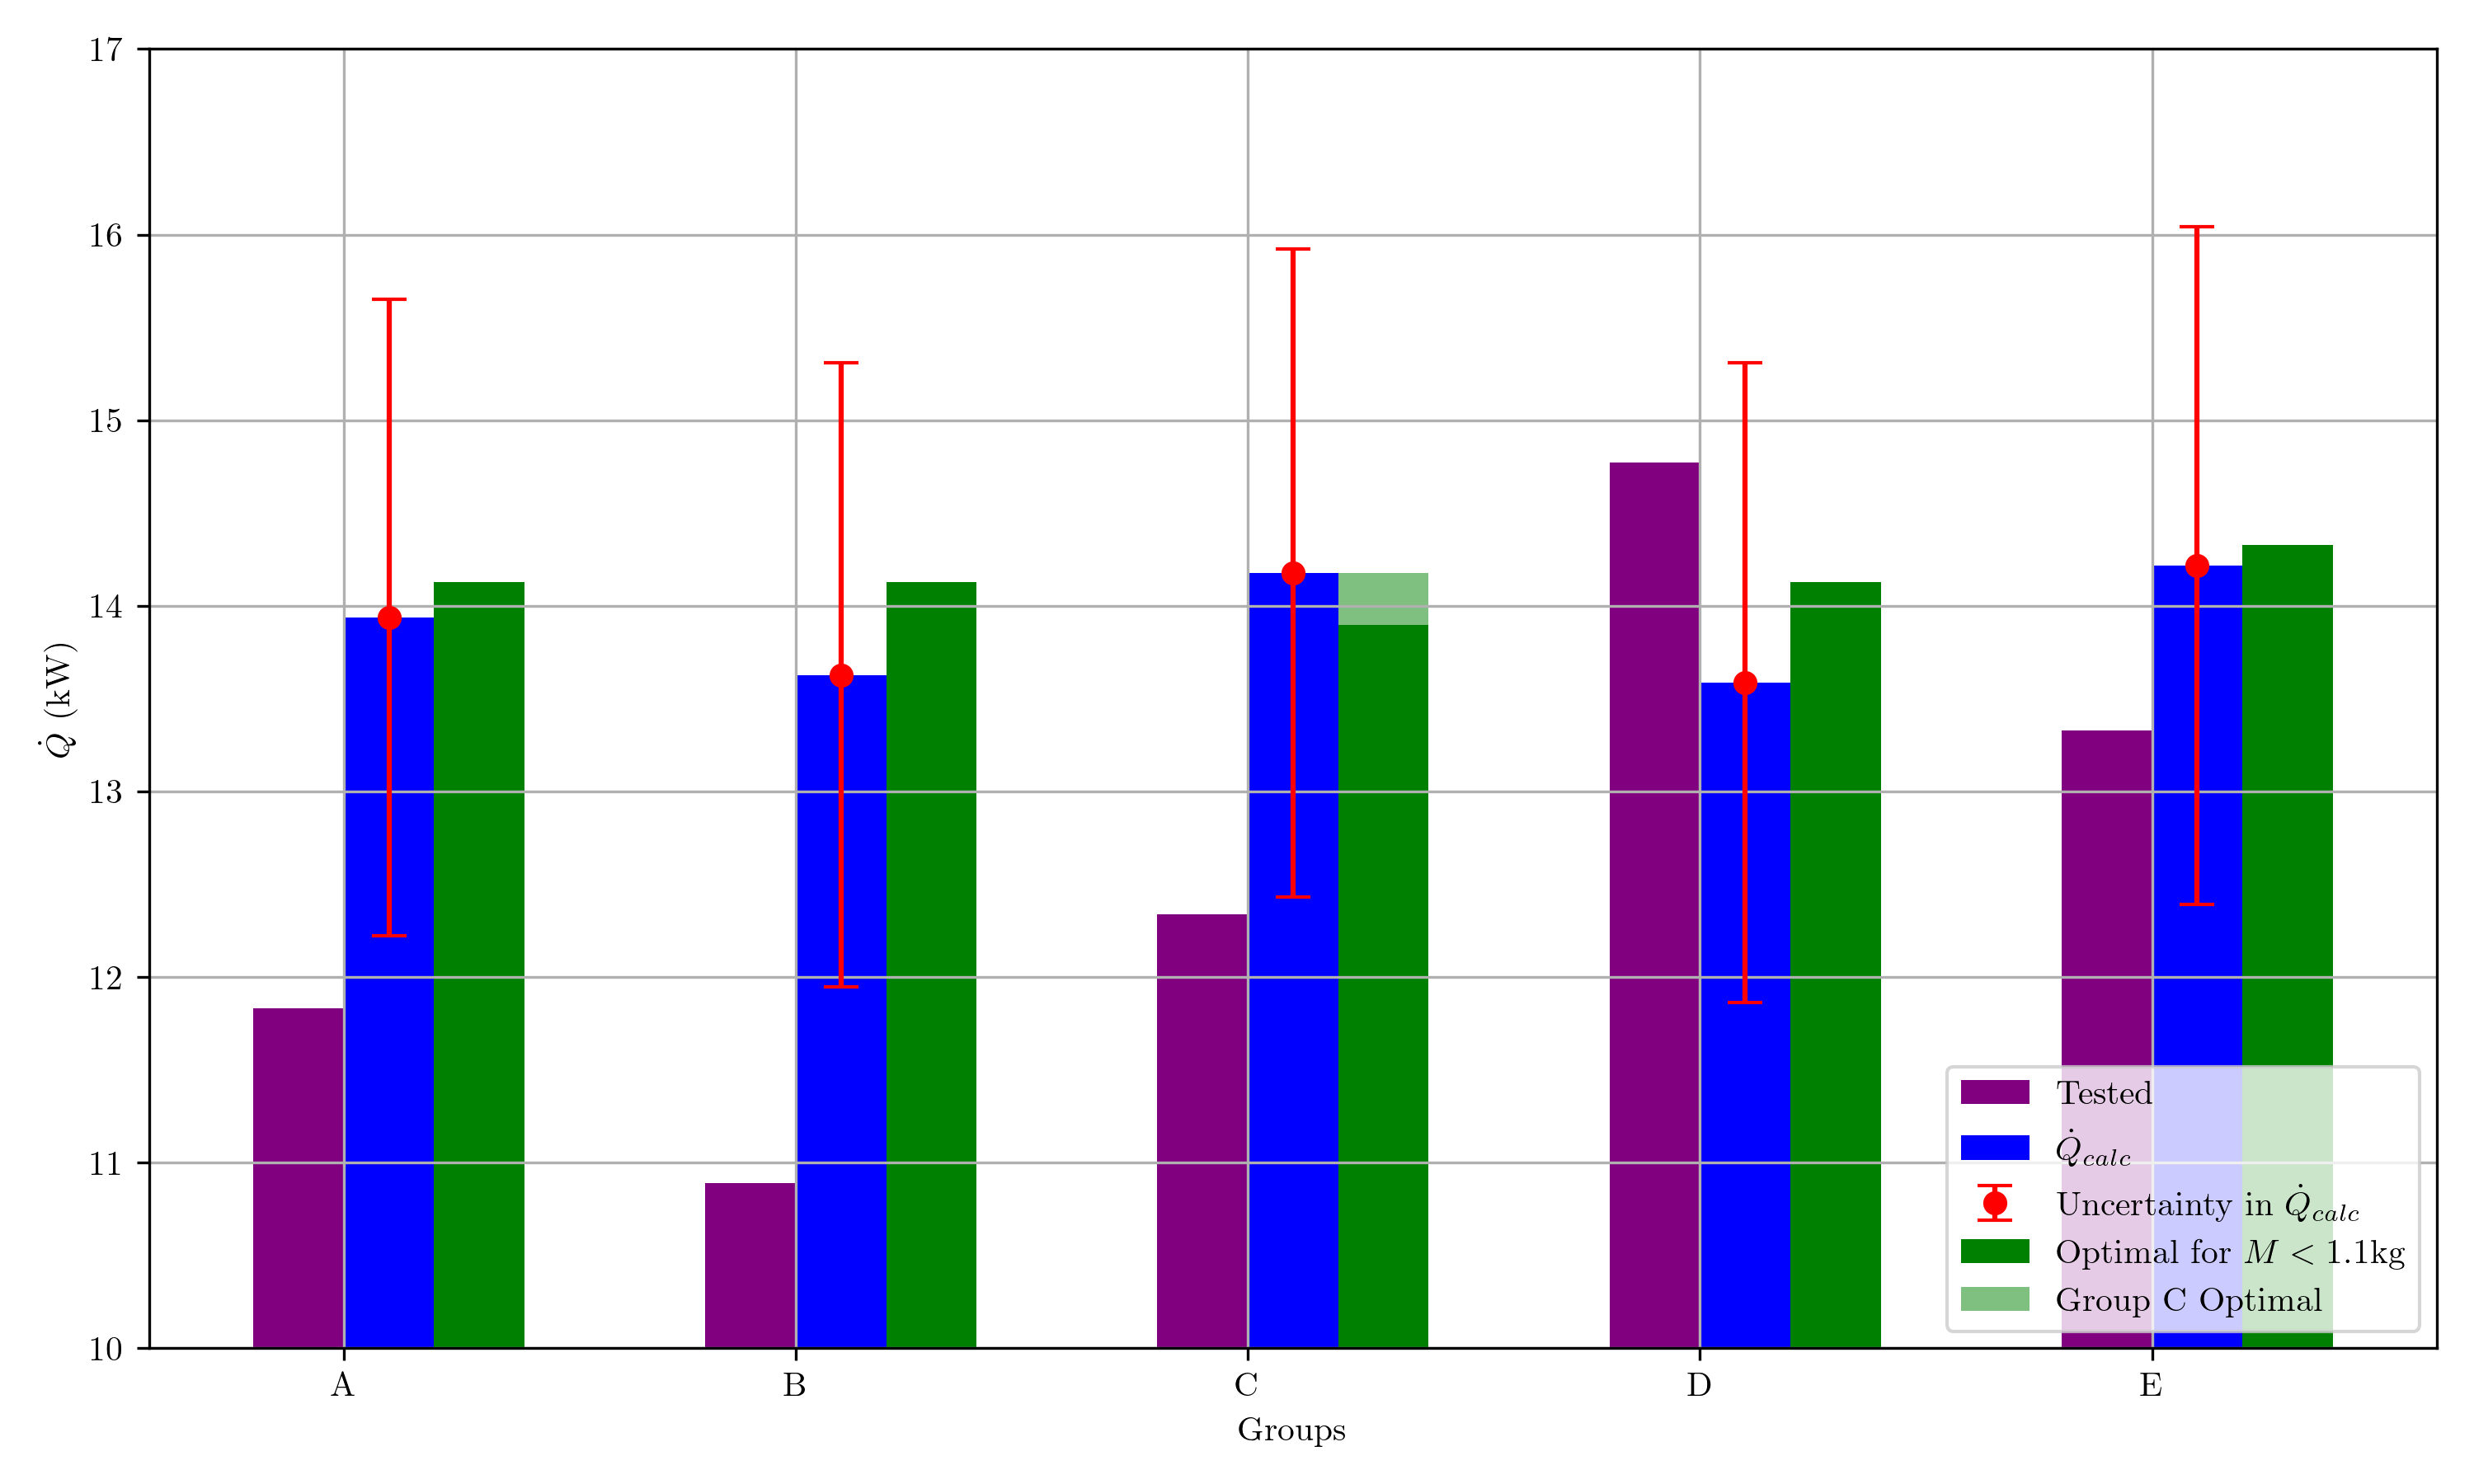
\includegraphics[width=0.99\textwidth]{2024_results.png}
        \captionof{figure}{$\dot{Q}$ results}
        \label{fig:Qdot_results} 
    \end{subfigure}
    \begin{subfigure}{0.8\textwidth}
        \centering
        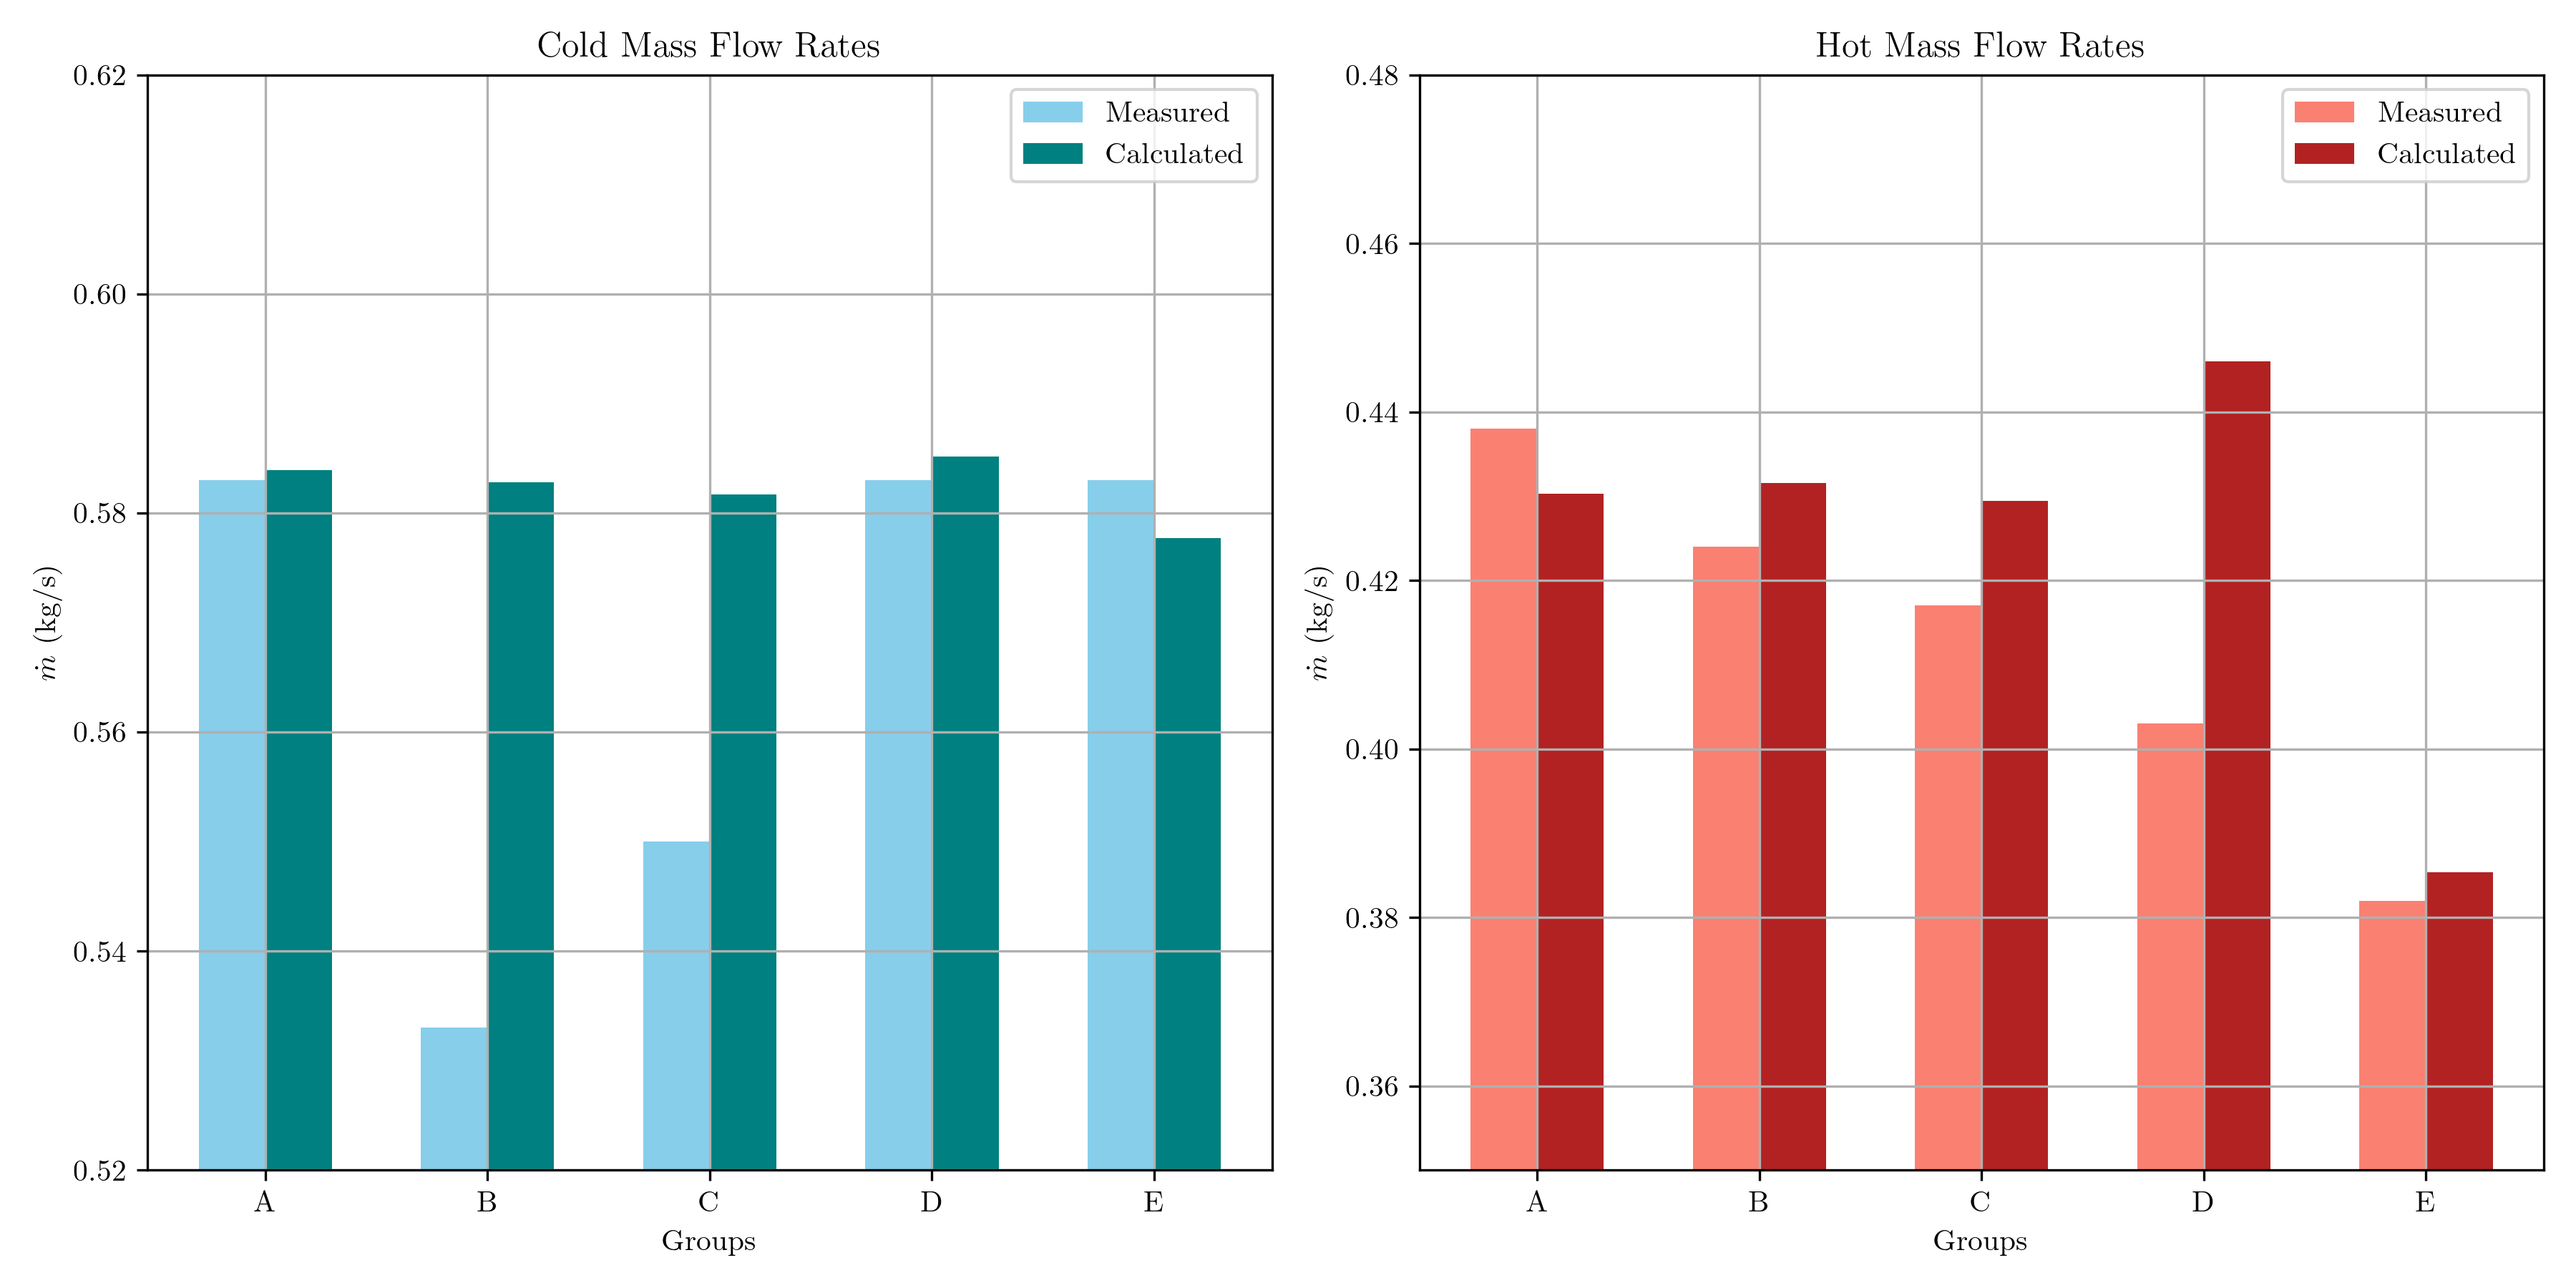
\includegraphics[width=0.99\textwidth]{2024_mass_flow_rates.png}
        \captionof{figure}{Mass flow rates of hot and cold sides for each group}
        \label{fig:mdot_results}
    \end{subfigure}
    \caption{Results}
\end{figure}

Figure \ref{fig:Qdot_results} shows the experimental results for the heat exchanger performance of each group.
Group D's heat exchanger performed the best, exceeding the calculated value by 

\newpage

\section{Future Work}
% more detailed fouling, comparison with bell delaware method
% additional constraints and design considerations for variety of applications:
% - optimal performance at a range of operating conditions
% - robustness to fouling and ease of maintenance
% - cost of materials and manufacturing at scale
% - ease of assembly and disassembly


\section{Recommendations}
% 

\section{Conclusion}

\end{document}